% flowcharts.tex - Các sơ đồ kiến trúc hệ thống
% Dựa trên source code thực tế của dự án
% Điều chỉnh khoảng cách và màu sắc theo mẫu

% ==============================================================================
% SƠ ĐỒ 1: KIẾN TRÚC TỔNG QUAN HỆ THỐNG MICROSERVICES
% ==============================================================================
\section{Sơ đồ kiến trúc tổng quan}
\label{sec:overall-architecture}

Sơ đồ \ref{fig:system-architecture} thể hiện kiến trúc tổng quan của hệ thống Crypto Analytics Platform với 4 microservices: Auth Service, Market Service, Crawler Service, AI Service, kết nối qua Kafka message broker.

\begin{figure}[H]
\centering
\begin{tikzpicture}[
    node distance=1.5cm,
    box/.style={rectangle, draw, minimum width=2.8cm, minimum height=0.9cm, align=center, font=\small, rounded corners}
]

% User
\node[box, fill=green!30] (user) {Người dùng\\Browser};

% Frontend
\node[box, fill=green!20, below=1.2cm of user] (fe) {Frontend\\React + Vite + TailwindCSS};

% Services Row
\node[box, fill=orange!30, below left=1.5cm and 2.5cm of fe] (auth) {Auth Service\\Golang\\Port: 8081};
\node[box, fill=orange!20, below=1.5cm of fe] (market) {Market Service\\Golang + WebSocket\\Port: 8082};
\node[box, fill=purple!30, below right=1.5cm and 2.5cm of fe] (crawler) {Crawler Service\\Golang\\Port: 8083};

% Kafka
\node[box, fill=yellow!30, below=3.5cm of fe] (kafka) {Kafka\\Message Broker\\Port: 9092};

% AI Service
\node[box, fill=red!30, below=1.2cm of kafka] (ai) {AI Service\\Python + FinBERT\\Port: 5000};

% Database
\node[box, fill=gray!30, below=1.2cm of ai] (db) {PostgreSQL\\cryptodb\\Port: 5432};

% External
\node[box, fill=cyan!30, right=1.5cm of market] (binance) {Binance\\WebSocket API};
\node[box, fill=cyan!20, right=1.5cm of crawler] (rss) {RSS Feeds\\News Sources};

% Arrows
\draw[->, thick] (user) -- (fe);
\draw[<->, thick] (fe) -- (auth);
\draw[<->, thick] (fe) -- (market);
\draw[->, thick] (fe) -- (crawler);
\draw[->, thick] (market) -- (binance);
\draw[->, thick] (crawler) -- (rss);
\draw[->, thick] (market) -- (kafka);
\draw[->, thick] (crawler) -- (kafka);
\draw[->, thick] (kafka) -- (ai);
\draw[->, thick] (auth) |- (db);
\draw[->, thick] (market) |- (db);
\draw[->, thick] (crawler) |- (db);
\draw[->, thick] (ai) -- (db);

% Layer labels
\node[font=\footnotesize, gray, left=0.3cm of user] {Client};
\node[font=\footnotesize, gray, left=0.3cm of auth] {Services};
\node[font=\footnotesize, gray, left=0.3cm of kafka] {Messaging};
\node[font=\footnotesize, gray, left=0.3cm of db] {Data};

\end{tikzpicture}
\caption{Kiến trúc Microservices Crypto Analytics Platform}
\label{fig:system-architecture}
\end{figure}

% ==============================================================================
% SƠ ĐỒ 2: WEBSOCKET HUB PATTERN - XỬ LÝ 1000+ CLIENTS
% ==============================================================================
\section{Sơ đồ WebSocket Hub Pattern}
\label{sec:websocket-hub-flow}

Sơ đồ \ref{fig:websocket-hub} mô tả chi tiết luồng xử lý của WebSocket Hub pattern được triển khai trong file \texttt{market-service/pkg/websocket/hub.go}. Pattern này cho phép hệ thống xử lý đồng thời 1000+ clients với topic-based subscription.

\begin{figure}[H]
\centering
\begin{tikzpicture}[
    node distance=1.5cm,
    box/.style={rectangle, draw, minimum width=2.8cm, minimum height=0.9cm, align=center, font=\small, rounded corners},
    decision/.style={diamond, draw, minimum width=2cm, align=center, font=\small, aspect=2},
    channel/.style={ellipse, draw, minimum width=2.5cm, align=center, font=\small}
]

% Hub struct
\node[box, fill=green!30] (hub) {Hub Struct\\topics map[string]map};

% Channels
\node[channel, fill=blue!20, below left=1.8cm and 2cm of hub] (regchan) {Register\\Channel};
\node[channel, fill=orange!20, below=1.8cm of hub] (subchan) {Subscribe\\Channel};
\node[channel, fill=purple!20, below right=1.8cm and 2cm of hub] (broadcastchan) {Broadcast\\Channel};

% Select Loop
\node[decision, fill=yellow!30, below=3.5cm of hub] (select) {select\\loop};

% Processes
\node[box, fill=blue!30, below left=2cm and 2cm of select] (register) {Register Client\\Log connection};
\node[box, fill=orange!30, below=2cm of select] (subscribe) {Subscribe Topic\\topics[topic][client]=true};
\node[box, fill=purple!30, below right=2cm and 2cm of select] (broadcast) {Broadcast\\topic -> clients\\client.send <- data};

% Client struct
\node[box, fill=cyan!30, left=1.5cm of regchan] (client) {Client\\hub, conn, send};

% Goroutines
\node[box, fill=green!20, below=1.5cm of register] (readpump) {ReadPump\\ParseJSON\\Handle subscribe};
\node[box, fill=pink!30, below=1.5cm of subscribe] (writepump) {WritePump\\WriteJSON\\to client};

% WebSocket Connection
\node[box, fill=gray!30, below=1.5cm of broadcast] (wsconn) {WSConn\\gorilla/websocket};

% Arrows
\draw[->, thick] (client) -- (regchan);
\draw[->, thick] (hub) -- (regchan);
\draw[->, thick] (hub) -- (subchan);
\draw[->, thick] (hub) -- (broadcastchan);

\draw[->, thick] (regchan) -- (select);
\draw[->, thick] (subchan) -- (select);
\draw[->, thick] (broadcastchan) -- (select);

\draw[->, thick] (select) -- node[left, font=\footnotesize] {case} (register);
\draw[->, thick] (select) -- (subscribe);
\draw[->, thick] (select) -- node[right, font=\footnotesize] {case} (broadcast);

\draw[->, thick] (register) -- (readpump);
\draw[->, thick] (subscribe) -- (writepump);
\draw[->, thick] (broadcast) -- (wsconn);

% Config labels
\node[font=\footnotesize, align=left, fill=white, draw=gray!50, rounded corners] at (6, -4) {
Topic format:\\
market:BTCUSDT:1h\\
market:ETHUSDT:1m
};

% Goroutines
\node[box, fill=green!20, below=1.5cm of register] (readpump) {ReadPump\\SetPongHandler\\ReadMessage};
\node[box, fill=pink!30, below=1.5cm of unregister] (writepump) {WritePump\\ticker(54s)\\WriteMessage};

% WebSocket Connection
\node[box, fill=gray!30, below=1.5cm of broadcast] (wsconn) {WSConn\\gorilla/websocket};

% Arrows
\draw[->, thick] (client) -- (regchan);
\draw[->, thick] (hub) -- (regchan);
\draw[->, thick] (hub) -- (unregchan);
\draw[->, thick] (hub) -- (broadcastchan);

\draw[->, thick] (regchan) -- (select);
\draw[->, thick] (unregchan) -- (select);
\draw[->, thick] (broadcastchan) -- (select);

\draw[->, thick] (select) -- node[left, font=\footnotesize] {case} (register);
\draw[->, thick] (select) -- (unregister);
\draw[->, thick] (select) -- node[right, font=\footnotesize] {case} (broadcast);

\draw[->, thick] (register) -- (readpump);
\draw[->, thick] (unregister) -- (writepump);
\draw[->, thick] (broadcast) -- (wsconn);

% Config labels
\node[font=\footnotesize, align=left, fill=white, draw=gray!50, rounded corners] at (6, -4) {
writeWait: 10s\\
pongWait: 60s\\
pingPeriod: 54s\\
maxMsgSize: 512KB
};

\end{tikzpicture}
\caption{WebSocket Hub Pattern - Xử lý đồng thời 1000+ clients}
\label{fig:websocket-hub}
\end{figure}

% ==============================================================================
% SƠ ĐỒ 3: LUỒNG XỬ LÝ WEBSOCKET CLIENT CONNECTION
% ==============================================================================
\section{Luồng kết nối WebSocket Client}
\label{sec:websocket-client-flow}

\begin{figure}[H]
\centering
\begin{tikzpicture}[
    node distance=1.2cm,
    startstop/.style={ellipse, draw, minimum width=2.5cm, align=center, font=\small},
    box/.style={rectangle, draw, minimum width=3.5cm, minimum height=0.9cm, align=center, font=\small, rounded corners},
    decision/.style={diamond, draw, minimum width=2cm, align=center, font=\small, aspect=2}
]

% Start
\node[startstop, fill=green!30] (start) {Client Connect};

% Frontend useWebSocket
\node[box, fill=green!20, below=1.2cm of start] (usews) {useWebSocket(url)\\new WebSocket()};

% Backend HandleWebSocket
\node[box, fill=orange!30, below=1.2cm of usews] (upgrade) {upgrader.Upgrade()\\CheckOrigin: true};

% Create Client
\node[box, fill=blue!30, below=1.2cm of upgrade] (createclient) {Create Client\\Hub, Pair, Conn, Send};

% Register
\node[box, fill=purple!30, below=1.2cm of createclient] (register) {hub.Register <- client};

% Fork goroutines
\node[box, fill=cyan!30, below=1.2cm of register] (goroutine) {go ReadPump()\\go WritePump()};

% ReadPump loop
\node[decision, fill=yellow!30, below left=1.5cm and 2.5cm of goroutine] (readloop) {Read\\Message?};
\node[box, fill=blue!20, below=1.5cm of readloop] (pong) {SetPongHandler\\ResetDeadline};

% WritePump loop
\node[decision, fill=yellow!30, below right=1.5cm and 2.5cm of goroutine] (writeloop) {Send\\Channel?};
\node[box, fill=orange!20, below=1.5cm of writeloop] (write) {WriteJSON\\to client};
\node[box, fill=pink!30, below=1.2cm of write] (ping) {Ping every 54s\\ticker.C};

% Close
\node[box, fill=red!30, below=3cm of goroutine] (close) {hub.Unregister <- client\\conn.Close()};
\node[startstop, fill=red!20, below=1.2cm of close] (end) {Disconnected};

% Arrows
\draw[->, thick] (start) -- (usews);
\draw[->, thick] (usews) -- (upgrade);
\draw[->, thick] (upgrade) -- (createclient);
\draw[->, thick] (createclient) -- (register);
\draw[->, thick] (register) -- (goroutine);
\draw[->, thick] (goroutine) -| (readloop);
\draw[->, thick] (goroutine) -| (writeloop);

\draw[->, thick] (readloop) -- node[left, font=\footnotesize] {yes} (pong);
\draw[->, thick] (pong.west) -- ++(-0.8, 0) |- (readloop.west);
\draw[->, thick] (readloop.south) -- ++(0, -0.5) -- ++(-2, 0) node[above, font=\footnotesize] {error} |- (close.west);

\draw[->, thick] (writeloop) -- node[right, font=\footnotesize] {data} (write);
\draw[->, thick] (write.east) -- ++(0.8, 0) |- (writeloop.east);
\draw[->, thick] (writeloop.south) -- ++(0, -0.5) -- (ping);
\draw[->, thick] (ping.east) -- ++(1, 0) |- (writeloop.east);

\draw[->, thick] (close) -- (end);

\end{tikzpicture}
\caption{Luồng kết nối và xử lý WebSocket Client}
\label{fig:websocket-client-flow}
\end{figure}

% ==============================================================================
% SƠ ĐỒ 4: CRAWLER SERVICE FLOW - THU THẬP TIN TỨC
% ==============================================================================
\section{Sơ đồ Crawler Service}
\label{sec:crawler-flow}

Sơ đồ \ref{fig:crawler-flow} mô tả luồng hoạt động của Crawler Service, được triển khai trong \texttt{services/crawler/main.py}. Service này tự động thu thập tin tức mỗi 30 phút với khả năng tự học cấu trúc HTML và retry với exponential backoff.

\begin{figure}[H]
\centering
\resizebox{0.85\textwidth}{!}{%
\begin{tikzpicture}[
    node distance=1.0cm and 1.5cm,
    startstop/.style={ellipse, draw, minimum width=1.4cm, align=center, font=\scriptsize},
    box/.style={rectangle, draw, minimum width=1.6cm, minimum height=0.6cm, align=center, font=\scriptsize, rounded corners},
    decision/.style={diamond, draw, minimum width=1.2cm, aspect=1.8, align=center, font=\scriptsize, inner sep=0pt},
    line/.style={draw, ->, >=stealth, thick}
]

% Main Spine (Vertical)
\node[startstop, fill=green!30] (start) {Schedule\\30min};
\node[box, fill=blue!30, below=0.8cm of start] (getsrc) {Get News\\Sources};
\node[decision, fill=yellow!30, below=0.8cm of getsrc] (loopsrc) {Have\\Source?};

\node[box, fill=orange!30, below=1.2cm of loopsrc] (fetch) {requests.get()};
\node[decision, fill=yellow!30, below=0.8cm of fetch] (error) {Error?};

\node[box, fill=purple!30, below=1.0cm of error] (learn) {learn\_structure()};
\node[box, fill=blue!20, below=0.8cm of learn] (soup) {soup.select()};

\node[decision, fill=yellow!30, below=0.8cm of soup] (loopart) {Have\\Article?};
\node[decision, fill=yellow!30, below=1.2cm of loopart] (exists) {In DB?};

% Side Branches (Right)
\node[box, fill=red!30, right=2cm of fetch] (backoff) {Backoff\\$2^n$s};
\node[box, fill=cyan!30, right=2cm of exists] (extract) {extract\_news()};
\node[box, fill=gray!30, below=0.8cm of extract] (save) {INSERT\\news};

% End Node (Left of Loop)
\node[startstop, fill=red!20, left=2.5cm of loopsrc] (end) {Complete};

% Connections

% 1. Start sequence
\draw[line] (start) -- (getsrc);
\draw[line] (getsrc) -- (loopsrc);

% 2. Source Loop -> Fetch
\draw[line] (loopsrc) -- node[right, font=\tiny] {yes} (fetch);

% 3. Fetch -> Error Handling
\draw[line] (fetch) -- (error);
\draw[line] (error) -- node[above, font=\tiny] {yes} (backoff);
\draw[line] (backoff) |- (fetch.east); % Loop back to fetch
\draw[line] (error) -- node[right, font=\tiny] {no} (learn);

% 4. Processing
\draw[line] (learn) -- (soup);
\draw[line] (soup) -- (loopart);

% 5. Article Loop -> DB Check
\draw[line] (loopart) -- node[right, font=\tiny] {yes} (exists);

% 6. Exists Logic
\draw[line] (exists) -- node[above, font=\tiny] {no} (extract);
\draw[line] (extract) -- (save);

% 7. Article Loop Backs
% Loop back if Exists=Yes (skip extract)
\draw[line] (exists.west) -- ++(-0.8, 0) |- node[near start, left, font=\tiny] {yes} (loopart.west);
% Loop back after Save (next article)
\draw[line] (save.east) -- ++(0.5, 0) |- (loopart.east);

% 8. Source Loop Back
% When articles done -> go to next source
\draw[line] (loopart.west) -- ++(-1.8, 0) |- node[near start, above, font=\tiny] {no/done} (loopsrc.west);

% 9. End
\draw[line] (loopsrc) -- node[above, font=\tiny] {no/done} (end);

\end{tikzpicture}%
}
\caption{Luồng hoạt động Crawler Service (Optimized Layout)}
\label{fig:crawler-flow}
\end{figure}

% ==============================================================================
% SƠ ĐỒ 5: AI SERVICE FLOW - PHÂN TÍCH VÀ DỰ ĐOÁN
% ==============================================================================
\section{Sơ đồ AI Analysis Service}
\label{sec:ai-service-flow}

Sơ đồ \ref{fig:ai-flow} mô tả pipeline phân tích AI của hệ thống, được triển khai trong \texttt{services/ai-service-python/}. Service này sử dụng FinBERT (English) và PhoBERT (Vietnamese) để phân tích sentiment đa ngôn ngữ, kết hợp với Gemini AI để phân tích CSS selectors.

\begin{figure}[H]
\centering
\resizebox{0.95\textwidth}{!}{%
\begin{tikzpicture}[
    node distance=0.8cm,
    startstop/.style={ellipse, draw, minimum width=1.8cm, align=center, font=\footnotesize},
    box/.style={rectangle, draw, minimum width=2.5cm, minimum height=0.65cm, align=center, font=\footnotesize, rounded corners},
    decision/.style={diamond, draw, minimum width=1.2cm, align=center, font=\footnotesize, aspect=1.8},
    data/.style={rectangle, draw, minimum width=2cm, minimum height=0.55cm, align=center, font=\footnotesize}
]

% Input
\node[startstop, fill=green!30] (start) {Kafka Message};

% Get news
\node[box, fill=blue!30, below=0.7cm of start] (getnews) {KafkaConsumer\\read\_message()};

% Language Detection
\node[decision, fill=yellow!30, below=0.8cm of getnews] (langdetect) {Language?};

% FinBERT Analysis (English)
\node[box, fill=purple!30, below left=0.9cm and 1.2cm of langdetect] (finbert) {FinBERT\\English Financial};

% PhoBERT Analysis (Vietnamese)
\node[box, fill=orange!30, below right=0.9cm and 1.2cm of langdetect] (phobert) {PhoBERT\\Vietnamese};

% Combine scores
\node[box, fill=cyan!30, below=2.2cm of langdetect] (analyze) {Analyze Sentiment\\+ Extract Keywords};

% Classify
\node[decision, fill=yellow!30, below=0.8cm of analyze] (classify) {Score?};

% Labels
\node[data, fill=green!30, below left=1cm and 1.5cm of classify] (positive) {positive\\$\geq$0.05};
\node[data, fill=gray!30, below=1cm of classify] (neutral) {neutral};
\node[data, fill=red!30, below right=1cm and 1.5cm of classify] (negative) {negative\\$\leq$-0.05};

% Update DB
\node[box, fill=blue!20, below=2.5cm of classify] (update) {UPDATE articles SET\\sentiment\_score, keywords};

% Attention Keywords
\node[box, fill=orange!20, below=0.7cm of update] (keywords) {Attention-based\\Keyword Extraction};

% Response
\node[startstop, fill=pink!30, below=0.7cm of keywords] (response) {Save to Database};

% Arrows
\draw[->, thick] (start) -- (getnews);
\draw[->, thick] (getnews) -- (langdetect);
\draw[->, thick] (langdetect) -| node[above, font=\tiny, pos=0.3] {en} (finbert);
\draw[->, thick] (langdetect) -| node[above, font=\tiny, pos=0.3] {vi} (phobert);
\draw[->, thick] (finbert) |- (analyze);
\draw[->, thick] (phobert) |- (analyze);
\draw[->, thick] (combine) -- (classify);

\draw[->, thick] (classify) -| node[above, font=\tiny, pos=0.3] {$\geq$0.05} (positive);
\draw[->, thick] (classify) -- (neutral);
\draw[->, thick] (classify) -| node[above, font=\tiny, pos=0.3] {$\leq$-0.05} (negative);

\draw[->, thick] (positive) |- (update);
\draw[->, thick] (neutral) -- (update);
\draw[->, thick] (negative) |- (update);

\draw[->, thick] (update) -- (keywords);
\draw[->, thick] (keywords) -- (response);

\end{tikzpicture}%
}
\caption{AI Analysis Pipeline - FinBERT/PhoBERT Sentiment Analysis}
\label{fig:ai-flow}
\end{figure}

% ==============================================================================
% SƠ ĐỒ 6: KAFKA MESSAGE FLOW
% ==============================================================================
\section{Sơ đồ Kafka Message Flow}
\label{sec:kafka-flow}

Sơ đồ \ref{fig:kafka-flow} mô tả luồng message giữa các services thông qua Kafka, được triển khai trong các file \texttt{kafka/producer.go} và \texttt{kafka/consumer.py}.

\begin{figure}[H]
\centering
\begin{tikzpicture}[
    node distance=1.3cm,
    startstop/.style={ellipse, draw, minimum width=2.5cm, align=center, font=\small},
    box/.style={rectangle, draw, minimum width=3.5cm, minimum height=0.9cm, align=center, font=\small, rounded corners},
    decision/.style={diamond, draw, minimum width=2cm, align=center, font=\small, aspect=2},
    topic/.style={rectangle, draw, minimum width=3cm, minimum height=0.8cm, align=center, font=\small, fill=yellow!30}
]

% Producers
\node[box, fill=orange!30] (crawler) {Crawler Service\\Golang};
\node[box, fill=blue!30, right=3cm of crawler] (market) {Market Service\\Golang};

% Kafka Topics
\node[topic, below=1.5cm of crawler] (topic1) {news\_new\_article};
\node[topic, below=0.8cm of topic1] (topic2) {news\_analyze\_rss\_structure};
\node[topic, below=0.8cm of topic2] (topic3) {news\_analyze\_css\_selector};
\node[topic, below=1.5cm of market] (topic4) {market\_price\_update};

% Kafka Broker
\node[box, fill=yellow!20, below=3.5cm of crawler, xshift=2cm] (kafka) {Kafka Broker\\Port: 9092};

% Consumer
\node[box, fill=red!30, below=1.5cm of kafka] (ai) {AI Service\\Python + FinBERT};

% Arrows - Producers to Topics
\draw[->, thick] (crawler) -- (topic1);
\draw[->, thick] (crawler) -- (topic2);
\draw[->, thick] (crawler) -- (topic3);
\draw[->, thick] (market) -- (topic4);

% Topics to Kafka
\draw[->, thick] (topic1) -- (kafka);
\draw[->, thick] (topic2) -- (kafka);
\draw[->, thick] (topic3) -- (kafka);
\draw[->, thick] (topic4) -- (kafka);

% Kafka to Consumer
\draw[->, thick] (kafka) -- (ai);

% Labels
\node[font=\footnotesize, align=left, fill=white, draw=gray!50, rounded corners] at (6.5, -3) {
Topics:\\
- Sentiment analysis\\
- CSS selector learn\\
- Price updates
};

\end{tikzpicture}
\caption{Kafka Message Flow giữa các Microservices}
\label{fig:kafka-flow}
\end{figure}

% ==============================================================================
% SƠ ĐỒ 7: FRONTEND REACT COMPONENT FLOW
% ==============================================================================
\section{Sơ đồ Frontend React Component}
\label{sec:frontend-flow}

Sơ đồ \ref{fig:frontend-flow} mô tả cấu trúc components của Frontend React, với focus vào Chart component sử dụng Lightweight Charts và WebSocket Context cho real-time updates.

\begin{figure}[H]
\centering
\begin{tikzpicture}[
    node distance=1.3cm,
    box/.style={rectangle, draw, minimum width=3cm, minimum height=0.9cm, align=center, font=\small, rounded corners}
]

% App.tsx
\node[box, fill=green!30] (app) {App.tsx\\BrowserRouter\\Routes};

% Pages Row
\node[box, fill=blue!30, below left=1.5cm and 2.5cm of app] (login) {Login.tsx\\Register.tsx};
\node[box, fill=blue!20, below=1.5cm of app] (dashboard) {Dashboard.tsx\\Chart + News};
\node[box, fill=orange!30, below right=1.5cm and 2.5cm of app] (sources) {Sources.tsx\\SourceForm.tsx};

% Components
\node[box, fill=cyan!30, below=3.5cm of app] (chart) {Chart.tsx\\Lightweight Charts};
\node[box, fill=pink!30, left=2cm of chart] (newssidebar) {NewsSidebar.tsx\\News List};
\node[box, fill=purple!30, right=2cm of chart] (prediction) {PredictionPanel.tsx\\AI Predictions};

% Context
\node[box, fill=yellow!30, below=1.5cm of chart] (wscontext) {WebSocketContext.tsx\\subscribe, unsubscribe};

% API
\node[box, fill=orange!20, below=1.5cm of wscontext] (apiclient) {api/client.ts\\axios instance};

% External
\node[box, fill=gray!30, below left=1.5cm and 2cm of apiclient] (authapi) {Auth Service\\:8081};
\node[box, fill=gray!30, below=1.5cm of apiclient] (marketapi) {Market Service\\:8082};
\node[box, fill=gray!30, below right=1.5cm and 2cm of apiclient] (crawlerapi) {Crawler Service\\:8083};

% Arrows
\draw[->, thick] (app) -| (login);
\draw[->, thick] (app) -- (dashboard);
\draw[->, thick] (app) -| (sources);

\draw[->, thick] (dashboard) -- (chart);
\draw[->, thick] (dashboard) -| (newssidebar);
\draw[->, thick] (dashboard) -| (prediction);

\draw[->, thick] (chart) -- (wscontext);
\draw[->, thick] (wscontext) -- (apiclient);
\draw[->, thick] (apiclient) -| (authapi);
\draw[->, thick] (apiclient) -- (marketapi);
\draw[->, thick] (apiclient) -| (crawlerapi);

\end{tikzpicture}
\caption{Frontend React Component Architecture}
\label{fig:frontend-flow}
\end{figure}

% ==============================================================================
% SƠ ĐỒ 8: AUTHENTICATION FLOW
% ==============================================================================
\section{Sơ đồ Authentication và Security}
\label{sec:auth-flow}

Sơ đồ \ref{fig:auth-flow} mô tả luồng xác thực người dùng với JWT Access Token và Refresh Token, được triển khai trong \texttt{auth-service/}.

\begin{figure}[H]
\centering
\begin{tikzpicture}[
    node distance=1.2cm,
    startstop/.style={ellipse, draw, minimum width=2.2cm, align=center, font=\small},
    box/.style={rectangle, draw, minimum width=3.2cm, minimum height=0.9cm, align=center, font=\small, rounded corners},
    decision/.style={diamond, draw, minimum width=1.8cm, align=center, font=\small, aspect=2},
    data/.style={rectangle, draw, minimum width=2.8cm, minimum height=0.8cm, align=center, font=\small}
]

% User action
\node[startstop, fill=green!30] (start) {User Login};

% Login endpoint
\node[box, fill=blue!30, below=1.2cm of start] (login) {POST /auth/login\\email, password};

% Validate
\node[decision, fill=yellow!30, below=1.2cm of login] (validate) {Valid\\Creds?};

% Hash check
\node[box, fill=orange!30, right=2.5cm of validate] (hash) {bcrypt.Compare\\PasswordHash};

% Generate token
\node[box, fill=purple!30, below=1.5cm of validate] (gentoken) {GenerateAccessToken\\GenerateRefreshToken};

% Return error
\node[box, fill=red!30, left=2.5cm of validate] (error) {401 Unauthorized\\ErrInvalidCredentials};

% Save refresh token
\node[box, fill=pink!30, below=1.2cm of gentoken] (saverefresh) {Save RefreshToken\\to Database};

% Return token
\node[data, fill=green!20, below=1.2cm of saverefresh] (returntoken) {AuthResponse\\accessToken, refreshToken};

% Refresh flow
\node[box, fill=blue!20, below=1.2cm of returntoken] (refresh) {POST /auth/refresh\\refreshToken};

% Validate refresh
\node[decision, fill=yellow!30, below=1.2cm of refresh] (validaterefresh) {Token in\\DB?};

% Token rotation
\node[box, fill=cyan!30, below=1.5cm of validaterefresh] (rotate) {Token Rotation\\Delete old, Create new};

% Response
\node[startstop, fill=cyan!30, below=1.2cm of rotate] (end) {New Token Pair};

% Arrows
\draw[->, thick] (start) -- (login);
\draw[->, thick] (login) -- (validate);
\draw[->, thick] (validate) -- node[above, font=\footnotesize] {no} (error);
\draw[->, thick] (validate) -- node[above, font=\footnotesize] {check} (hash);
\draw[->, thick] (hash) |- (gentoken);
\draw[->, thick] (validate) -- node[left, font=\footnotesize] {yes} (gentoken);
\draw[->, thick] (gentoken) -- (saverefresh);
\draw[->, thick] (saverefresh) -- (returntoken);
\draw[->, thick] (returntoken) -- (refresh);
\draw[->, thick] (refresh) -- (validaterefresh);
\draw[->, thick] (validaterefresh) -- node[left, font=\footnotesize] {yes} (rotate);
\draw[->, thick] (validaterefresh.west) -- ++(-1.5, 0) node[above, font=\footnotesize] {no} |- (error);
\draw[->, thick] (rotate) -- (end);

\end{tikzpicture}
\caption{Authentication Flow với JWT + Refresh Token}
\label{fig:auth-flow}
\end{figure}

% ==============================================================================
% SƠ ĐỒ 9: DOCKER COMPOSE ORCHESTRATION
% ==============================================================================
\section{Sơ đồ Docker Compose Orchestration}
\label{sec:docker-flow}

Sơ đồ \ref{fig:docker-flow} mô tả cách các container được orchestrate bằng Docker Compose với Kafka message broker.

\begin{figure}[H]
\centering
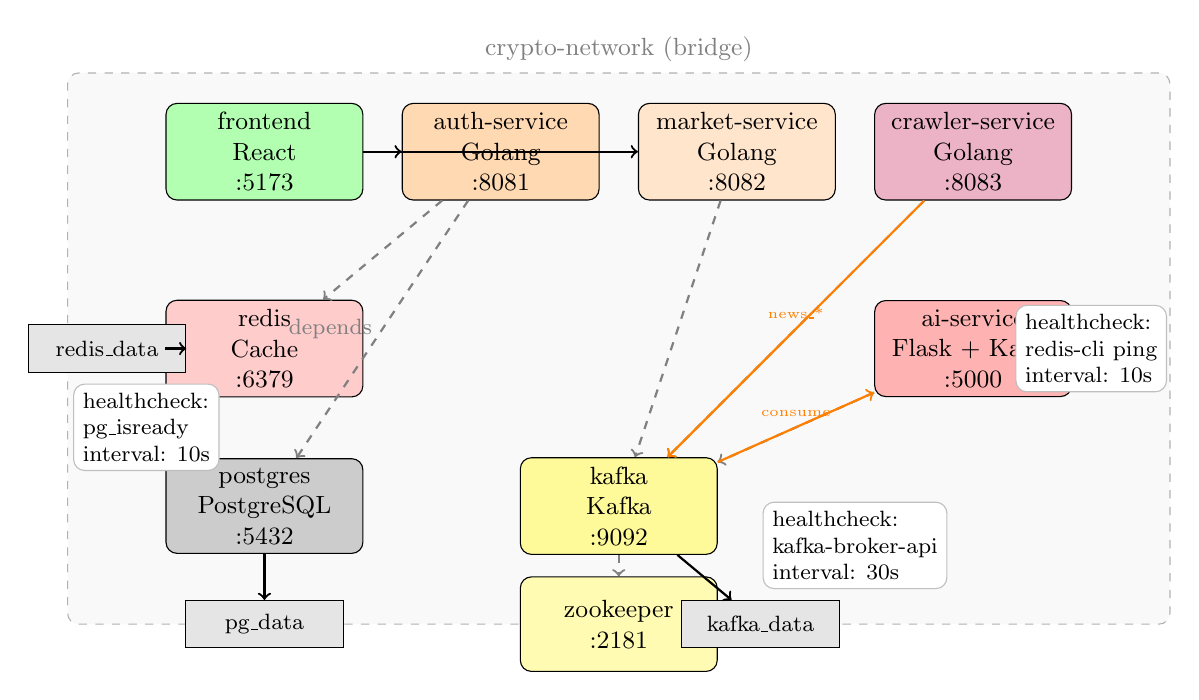
\begin{tikzpicture}[
    node distance=1.5cm,
    box/.style={rectangle, draw, minimum width=2.5cm, minimum height=1.2cm, align=center, font=\small, rounded corners},
    network/.style={rectangle, draw=gray!60, fill=gray!5, minimum width=14cm, minimum height=7cm, align=center, font=\small, dashed, rounded corners},
    volume/.style={rectangle, draw, minimum width=2cm, minimum height=0.6cm, align=center, font=\footnotesize}
]

% Network box
\node[network] (network) at (0, 0) {};
\node[font=\small, gray] at (0, 3.8) {crypto-network (bridge)};

% Containers - Top row
\node[box, fill=green!30] (frontend) at (-4.5, 2.5) {frontend\\React\\:5173};

\node[box, fill=orange!30] (authservice) at (-1.5, 2.5) {auth-service\\Golang\\:8081};

\node[box, fill=orange!20] (marketservice) at (1.5, 2.5) {market-service\\Golang\\:8082};

\node[box, fill=purple!30] (crawler) at (4.5, 2.5) {crawler-service\\Golang\\:8083};

% Redis
\node[box, fill=red!20] (redis) at (-4.5, 0) {redis\\Cache\\:6379};
\node[volume, fill=gray!20] (redisdata) at (-6.5, 0) {redis\_data};

% AI Service
\node[box, fill=red!30] (aiservice) at (4.5, 0) {ai-service\\Flask + Kafka\\:5000};

\node[box, fill=gray!40] (postgres) at (-4.5, -2) {postgres\\PostgreSQL\\:5432};
\node[box, fill=yellow!40] (kafka) at (0, -2) {kafka\\Kafka\\:9092};
\node[box, fill=yellow!30] (zookeeper) at (0, -3.5) {zookeeper\\:2181};

% Volumes
\node[volume, fill=gray!20] (pgdata) at (-4.5, -3.5) {pg\_data};
\node[volume, fill=gray!20] (kafkadata) at (1.8, -3.5) {kafka\_data};

% Dependencies
\draw[->, thick, dashed, gray] (authservice) -- node[left, font=\footnotesize] {depends} (postgres);
\draw[->, thick, dashed, gray] (authservice) -- (redis);
\draw[->, thick, dashed, gray] (marketservice) -- (kafka);
\draw[->, thick, dashed, gray] (crawler) -- (kafka);
\draw[->, thick, dashed, gray] (aiservice) -- (kafka);
\draw[->, thick, dashed, gray] (kafka) -- (zookeeper);

% Kafka Topic arrows
\draw[->, thick, orange] (crawler) -- node[above, font=\tiny] {news\_*} (kafka);
\draw[->, thick, orange] (kafka) -- node[above, font=\tiny] {consume} (aiservice);

% Connections
\draw[->, thick] (frontend) -- (authservice);
\draw[->, thick] (frontend) -- (marketservice);
\draw[->, thick] (postgres) -- (pgdata);
\draw[->, thick] (redis) -- (redisdata);
\draw[->, thick] (kafka) -- (kafkadata);

% Health checks
\node[font=\footnotesize, align=left, fill=white, draw=gray!50, rounded corners] at (-6, -1) {
healthcheck:\\
pg\_isready\\
interval: 10s
};
\node[font=\footnotesize, align=left, fill=white, draw=gray!50, rounded corners] at (6, 0) {
healthcheck:\\
redis-cli ping\\
interval: 10s
};
\node[font=\footnotesize, align=left, fill=white, draw=gray!50, rounded corners] at (3, -2.5) {
healthcheck:\\
kafka-broker-api\\
interval: 30s
};

\end{tikzpicture}
\caption{Docker Compose Container Orchestration với Kafka Message Broker}
\label{fig:docker-flow}
\end{figure}

% ==============================================================================
% SƠ ĐỒ 10: DATA FLOW TỔNG HỢP
% ==============================================================================
\section{Sơ đồ Data Flow Tổng hợp}
\label{sec:data-flow}

Sơ đồ \ref{fig:data-flow} tổng hợp luồng dữ liệu từ nguồn bên ngoài (Binance, News Sources) đến người dùng cuối thông qua các layers của hệ thống với Kafka message broker.

\begin{figure}[H]
\centering
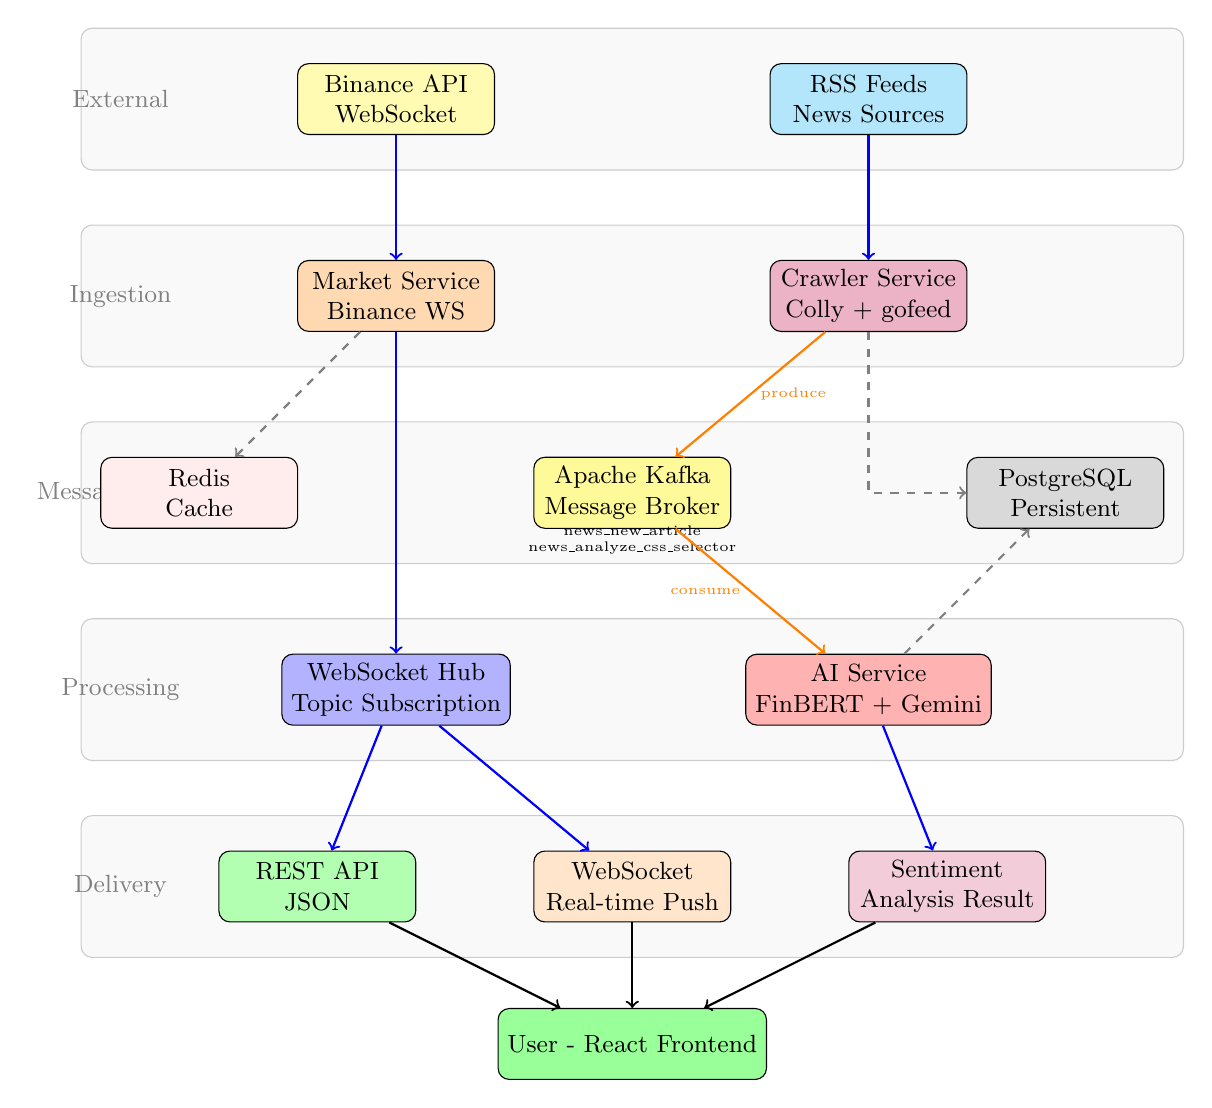
\begin{tikzpicture}[
    node distance=1.3cm,
    box/.style={rectangle, draw, minimum width=2.5cm, minimum height=0.9cm, align=center, font=\small, rounded corners},
    layer/.style={rectangle, draw=gray!40, fill=gray!5, minimum width=14cm, minimum height=1.8cm, rounded corners}
]

% Layer backgrounds
\node[layer] at (0, 5) {};
\node[layer] at (0, 2.5) {};
\node[layer] at (0, 0) {};
\node[layer] at (0, -2.5) {};
\node[layer] at (0, -5) {};

% Layer labels
\node[font=\small, gray] at (-6.5, 5) {External};
\node[font=\small, gray] at (-6.5, 2.5) {Ingestion};
\node[font=\small, gray] at (-6.5, 0) {Message\\Broker};
\node[font=\small, gray] at (-6.5, -2.5) {Processing};
\node[font=\small, gray] at (-6.5, -5) {Delivery};

% External sources
\node[box, fill=yellow!30] (binance) at (-3, 5) {Binance API\\WebSocket};
\node[box, fill=cyan!30] (newssrc) at (3, 5) {RSS Feeds\\News Sources};

% Ingestion layer
\node[box, fill=orange!30] (marketservice) at (-3, 2.5) {Market Service\\Binance WS};
\node[box, fill=purple!30] (crawler) at (3, 2.5) {Crawler Service\\Colly + gofeed};

% Message Broker layer
\node[box, fill=yellow!40] (kafka) at (0, 0) {Apache Kafka\\Message Broker};
\node[font=\tiny, align=center] at (0, -0.6) {news\_new\_article\\news\_analyze\_css\_selector};

% Processing layer
\node[box, fill=blue!30] (websockethub) at (-3, -2.5) {WebSocket Hub\\Topic Subscription};
\node[box, fill=red!30] (aiservice) at (3, -2.5) {AI Service\\FinBERT + Gemini};

% Delivery layer
\node[box, fill=green!30] (restapi) at (-4, -5) {REST API\\JSON};
\node[box, fill=orange!20] (realtime) at (0, -5) {WebSocket\\Real-time Push};
\node[box, fill=purple!20] (sentiment) at (4, -5) {Sentiment\\Analysis Result};

% User
\node[box, fill=green!40] (user) at (0, -7) {User - React Frontend};

% Storage (side)
\node[box, fill=pink!30] (redis) at (-5.5, 0) {Redis\\Cache};
\node[box, fill=gray!30] (postgres) at (5.5, 0) {PostgreSQL\\Persistent};

% Arrows - External to Ingestion
\draw[->, thick, blue] (binance) -- (marketservice);
\draw[->, thick, blue] (newssrc) -- (crawler);

% Arrows - Ingestion to Kafka
\draw[->, thick, orange] (crawler) -- node[right, font=\tiny] {produce} (kafka);

% Arrows - Kafka to Processing
\draw[->, thick, orange] (kafka) -- node[left, font=\tiny] {consume} (aiservice);

% Arrows - Direct paths (Market Service)
\draw[->, thick, blue] (marketservice) -- (websockethub);
\draw[->, thick, gray, dashed] (marketservice) -- (redis);

% Arrows - Storage
\draw[->, thick, gray, dashed] (crawler) |- (postgres);
\draw[->, thick, gray, dashed] (aiservice) -- (postgres);

% Arrows - Processing to Delivery
\draw[->, thick, blue] (websockethub) -- (restapi);
\draw[->, thick, blue] (websockethub) -- (realtime);
\draw[->, thick, blue] (aiservice) -- (sentiment);

% Arrows - Delivery to User
\draw[->, thick] (restapi) -- (user);
\draw[->, thick] (realtime) -- (user);
\draw[->, thick] (sentiment) -- (user);

\end{tikzpicture}
\caption{Data Flow từ nguồn đến người dùng với Kafka Message Broker}
\label{fig:data-flow}
\end{figure}
